In this section, we briefly describe the problem of face fiducial detection and face
frontalization along with related work.

\subsection{Face Fiducial Detection}

\begin{figure}[!ht]
  \centering
  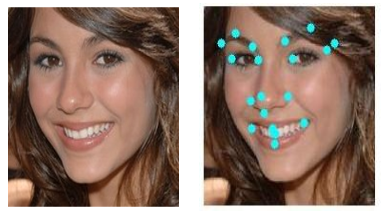
\includegraphics[width=9cm,height=4.5cm]{intro/figures/face_fid.png}
  \caption{}
  \label{fig:intro_face_fid}
\end{figure}

% - Problem  
%   - 
%   - 
% - Why challenge
% - Applications
%   - Gaze. Approx. Then starting point for finer details.
%   - Non verbal communication, intended target audience in a meeting
%   - In cars, to figure out driver is paying attention to the traffic on road
%   - Outside the car if the pedestrian is paying attention towards the car moving towards him
%   - 
% - Related work
%   - Global vs local modelling
%   - 
% 

Face fiducial detection is a problem of detecting key points on the face like 
eye corners, nose tip, mouth corners \etc., given a face image. It is a challenging
problem considering the influencing factors which include physical phenomena like camera distortion, projective
geometry, multisource lighting, biological appearance, facial expression, and the presence of
accessories like glasses and hats. 

Face fiducial detection is intrinsically linked with the head pose estimation, visual
gaze identification and emotion recognition. Head pose estimation 
can be considered as a more coarser level problem compared to that of fiducial detection
as it involves only inferfing the orientation of human head from the image. Head pose 
estimation comes for free if the fiducial detection problem is solved as it just a mapping
of location to orientation as they are highly correlated. Also, perceived gaze identification 
directly depends on the head pose at coarser level. Finer level estimation of eye direction
would require location of eyes, which can be inferred from fiducial detection.

Traditional face fiducial detection methods can be categorized into two types, namely regression
based method and template fitting method. Most of the methods iteratievely improvize the initial
 estimates by regression using image features. Support vector vegression has been employed by
Valstar \etal~\cite{FrancoisValstarMBP10} and Burgos-Artizzu \etal~\cite{artizzzuICCV13_COFW} employ cascaded fern regression. Image features 
like pixel-difference features and Haar-like features have been used. Since most of the regression
based methods start with an initial estimate of the locations, they are prone to propogate error with 
wrong initialization. Template based methods rely on pre-built templates to fit the input images.
Part based method~\cite{xhuCVPR12_wild} build model of each pre-defined parts and come to consensus using voting 
made by each part model on the input image using a tree representation, which can model the space constraints between parts.

\subsection{Face Frontalization}

\begin{figure}[!ht]
  \centering
  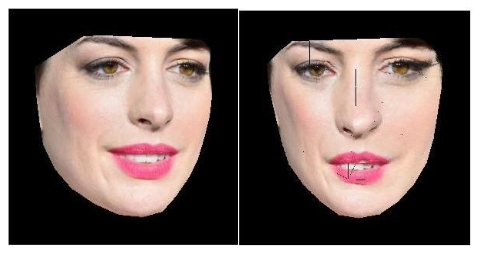
\includegraphics[width=9cm,height=4.5cm]{intro/figures/face_front.png}
  \caption{}
  \label{fig:intro_face_front}
\end{figure}

% - Problem
% -
% -
% - Apps
%   -  
%
% - Related Work

Face frontalization is a problem of synthesizing frontal view of the face given an non-frontal
face image. Synthesizing novel views of the face has been longstanding challenge in computer vision
mainly because of the potential application in graphics domain and recognition sytems. It is a challenging
problem considering faces with unconstrained scenarios with occlusions and specularities. 

Face recognition methods recently have claimed to reach the accuracy of that of humans even in
the unregulated, uncontrolled image settings. These approaches differ in addressing the problem 
of unconstrained settings. Unconstrained settings includes non-frontal pose, lighting, expression
variations and noise. One way to address the problem of non-frontal pose is to align the pose 
of the face to frontal pose to make the job easy for face recognition system. Pose correction 
technique can be used to correct the pose of any individual in a group photo if they are not looking
towards the camera. Addressing the problem of novel face pose can also be used in face 
reenactment systems where one can create a mimicry video of a person by replacing the original
actor.

General approach to synthesize novel face pose includes estimating a {\sc 3D} model~\cite{Wolf} of the face 
from a single image and then rendering the {\sc 3D} model from a different view angle on a {\sc 2D} image.
This approach intuitively seems good, but extracting {\sc 3D} information out of {\sc 2D} image is a
challenging problem. By relaxing certain constraint, one can think of assuming a generic {\sc 3D} model~\cite{DBLP:journals/corr/HassnerHPE14}
of a face and try to get an approximate estimate, but this leads to loss of crucial structural
information.

